\section{Technology Assessment}
\label{sec:technology}

Introduce in (sufficient) depth the key concepts and architecture of the chosen software technology. As part of this, you may consider using a running example to introduce the technology.

This part and other parts of the report probably need to refer to
figures. Figure~\ref{fig:framework} from \cite{brown:96} just
illustrates how a figure can be included in the report.

\begin{figure}[thb]
	\centering
	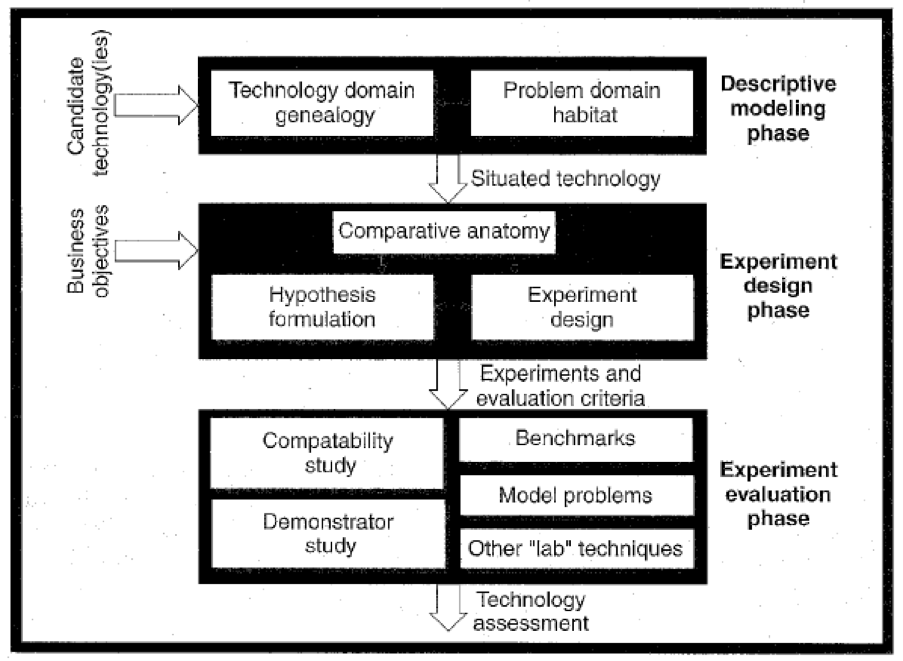
\includegraphics[scale=0.5]{figs/framework.png}
	\caption{Software technology evaluation framework.}
	\label{fig:framework}
\end{figure}

\subsection{Descriptive Modeling}
%write where the technology comes from, its history, its context and what problem it solves.
%Consider drawing a graph like in \cite{brown:96}.
OAuth 2.0 is a modern framework designed to facilitate secure access to resources on behalf of a user. It achieves this through a token-based system that delegates access using short-lived Access Tokens and optional Refresh Tokens. These tokens are associated with specific scopes, allowing fine-grained authorization to resources without exposing user credentials. OAuth 2.0's adoption as a web standard ensures compatibility with a wide range of APIs and systems, making it an ideal choice for securing FeedApp’s RESTful services.

API Keys represent an older, simpler approach to authenticating clients. An API Key is a static string generated by the server and assigned to a client. The client includes the key in each request to authenticate itself. While API Keys are easy to implement, they lack features such as token expiration, scope management, and secure delegation, making them less suitable for modern web applications.

Basic Authentication is a legacy method of authentication that sends a client’s username and password in every request’s header. While easy to implement, Basic Authentication poses significant security risks, as credentials are repeatedly transmitted and stored. It also lacks advanced features like token expiration or granular permission control, which are essential for FeedApp.

In this experiment, OAuth 2.0 is evaluated against API Keys and Basic Authentication to determine whether its complexity and capabilities justify its selection for FeedApp.

\subsection{Experiment Design}

\subsubsection*{Hypotheses}
This experiment evaluates OAuth 2.0's advantages over API Keys and Basic Authentication in the context of FeedApp’s requirements for secure, scalable, and flexible authorization. The comparison focuses on implementation complexity, security, performance, and scalability.

Hypotheses:


\begin{enumerate}
    \item \textbf{H1}: OAuth 2.0 provides superior security compared to API Keys and Basic Authentication, as it supports token expiration, revocation, and scoped access.

    \item \textbf{H2}: OAuth 2.0 demonstrates better scalability under high concurrent loads due to its token-based design and reduced reliance on static credentials.

    \item \textbf{H3}: OAuth 2.0 is more complex to implement than API Keys or Basic Authentication but provides better long-term maintainability and integration with external systems.
\end{enumerate}

Experimental Setup: Three identical prototypes are implemented, each securing the FeedApp API using a different authentication method:
\medskip

\noindent
Prototype A (OAuth 2.0):
Users authenticate using OAuth 2.0, and the client receives an Access Token with predefined scopes.
Prototype B (API Keys):
Users are assigned a static API Key that must be included in every request.
Prototype C (Basic Authentication):
Users authenticate with their username and password included in every request’s header.
Each prototype is tested under the following scenarios:
\medskip

\noindent
User login and token/key issuance.
Secured API calls, such as creating surveys and casting votes.
Concurrent requests simulating high user loads.
Evaluation Metrics:
\medskip

\noindent

Ease of Implementation:
\begin{itemize}
	\item  Time and effort required to implement each technology.
	\item  Developer feedback on challenges during configuration.
\end{itemize}
Security:
\begin{itemize}
	\item Protection against vulnerabilities (e.g., token theft, replay attacks).
	\item Support for advanced features like token expiration and revocation.
\end{itemize}
Performance:
\begin{itemize}
	\item  Latency in login flows and API requests.
	\item  System throughput under high-load scenarios.
\end{itemize}
Scalability:
\begin{itemize}
	\item  Handling of concurrent requests and performance consistency.
\end{itemize}
\subsection{Experiment Evaluation}

% Write about the results of your experiments, either via personal experience reports, quantitative benchmarks, a demonstrator case study, or a combination of multiple approaches.
The results are analyzed based on the defined metrics, focusing on how OAuth 2.0 compares to the alternatives in the context of FeedApp.

%For some reports, you may have to include a table with experimental
%results or other kinds of tables that, for instance, compare technologies. 
Table~\ref{tab:security-comparison} shows first hypothesis.

\begin{table}[h!]
\centering
\resizebox{\textwidth}{!}{%
\begin{tabular}{|l|c|c|c|}
\hline
\textbf{Security Feature}               & \textbf{OAuth 2.0}         & \textbf{Basic Authentication} & \textbf{API Key}       \\ \hline
\textbf{Token Expiration}               & Supported                  & Not Applicable                & Not Applicable         \\ \hline
\textbf{Token Revocation}               & Supported                  & Not Applicable                & Not Applicable         \\ \hline
\textbf{Replay Attack Prevention}       & Resistant (Nonce/Scopes)   & Weak                          & Weak                   \\ \hline
\textbf{Granular Permissions (Scopes)}  & Supported                  & Not Applicable                & Limited (via keys)     \\ \hline
\textbf{Credential Storage Risk}        & Low (Tokens Only)          & High (Requires Password)      & Medium (Static Key)    \\ \hline
\textbf{Ease of Key Rotation}           & Supported (Token Refresh)  & Not Applicable                & Limited (Manual Keys)  \\ \hline
\textbf{Transport Security Requirement} & TLS Required               & TLS Strongly Recommended      & TLS Strongly Recommended \\ \hline
\end{tabular}
}
\caption{Security Feature Comparison of Authentication Mechanisms}
\label{tab:security-comparison}
\end{table}



\begin{table}[h!]
\centering
\resizebox{\textwidth}{!}{%
\begin{tabular}{|l|c|c|p{6cm}|}
\hline
\textbf{Metric} & \textbf{Basic Authentication (100 VUs)} & \textbf{OAuth 2.0 (100 VUs)} & \textbf{Notes} \\ \hline
\textbf{Average Response Time} & 795.26 ms & TBD ms & OAuth is expected to be faster due to stateless token validation. \\ \hline
\textbf{Median Response Time} & 909.66 ms & TBD ms & Median reflects the typical experience for most users. \\ \hline
\textbf{90th Percentile Response Time} & 1.21 s & TBD ms & 90\% of requests complete within this time. \\ \hline
\textbf{95th Percentile Response Time} & 1.29 s & TBD ms & 95\% of requests complete within this time. \\ \hline
\textbf{Throughput} & 48.78 requests/second & TBD requests/second & Higher throughput suggests better scalability. \\ \hline
\textbf{Error Rate} & 0\% & 0\% & Both methods handle the load without dropping requests. \\ \hline
\textbf{CPU Utilization} & High & TBD & OAuth's lightweight token validation likely reduces CPU usage. \\ \hline
\textbf{Memory Utilization} & Moderate & TBD & OAuth avoids keeping session states or handling repeated logins. \\ \hline
\end{tabular}
}
\caption{Scalability Test Results}
\label{tab:scalability-results}
\end{table}


\begin{table}[h!]
\centering
\resizebox{\textwidth}{!}{%
\begin{tabular}{|l|c|c|c|}
\hline
\textbf{Metric}                          & \textbf{OAuth 2.0}         & \textbf{Basic Authentication} & \textbf{API Key}       \\ \hline
\textbf{Development Time (hrs)}          & 15 (Approx.)               & 5 (Approx.)                   & 5 (Approx.)            \\ \hline
\textbf{Code Complexity}                 & High                       & Low                           & Low                    \\ \hline
\textbf{Configuration Overhead}          & High (Token Server Needed) & Low                           & Medium                 \\ \hline
\textbf{Third-Party Integration Ease}    & Excellent                  & Poor                          & Moderate               \\ \hline
\textbf{Scalability Benefits}            & High                       & Low                           & Moderate               \\ \hline
\textbf{Maintainability (Long-Term)}     & High                       & Low                           & Medium                 \\ \hline
\textbf{Error-Prone Areas}               & Token Handling             & Password Storage              & API Key Leaks          \\ \hline
\end{tabular}
}
\caption{Implementation Complexity Comparison of Authentication Mechanisms}
\label{tab:implementation-complexity}
\end{table}



